\chapter{Proposed Design and Framework}


\section{System Design}

\begin{figure}[here]
\begin{center}	
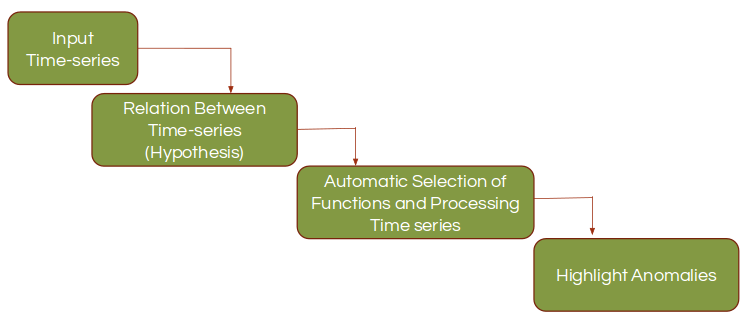
\includegraphics[scale=0.5]{System} 
\caption{System Design}
\label{fig:SystemDesign}
\end{center}
\end{figure}


So figure \ref{fig:SystemDesign} explains the overall design of the system and its modules. We have made some assumption regarding system as follows:

\begin{enumerate}

\item Given time series should be of the same time period.
\item Each time series should be present in different file.

\end{enumerate}

\subsection {Input Time-series}

Here, give option to user to input number of time series and accordingly, provide option to select time series in CSV format. Currently, we have thought of keeping restriction that CSV file should contain only one time series. Also, ask user whether he wants to smooth time series or not. Smoothing of time series will be done using Exponential Moving Average technique. $\alpha$  factor for same will be considered as \[ 2 / (1+ period) \].  Where period is considered as up to how much of previous values should have effect on today's value. By default, we have kept it as 14. If user has technical knowledge then option to select period can be provided.

\subsection {Relation Between Time-series (Hypothesis)}

Normal behavior of the time series should be stated somehow, so that we can detect anomaly in the data. So, to get this input from user, we will be providing \textit{n*n} matrix with some default value, where '\textit{n}' corresponds to the number of time series user gave as an input. Now by filling each cell in the matrix, user can specify the relation between any 2 time series as follows:


\begin{itemize}

\item \textbf{1:} Positive Correlation
\item \textbf{-1:} negative Correlation
\item \textbf{0:} Random Relation
\item \textbf{2:} User is not aware but is interested in finding relation, if exist any
\item \textbf{Default:} User is not aware of any relation and also any doesn’t exist according to user

\end{itemize}

If correlation exists, then we may also take input from user maximum lag factor to consider. If not provided any, then by default it will be taken as -15 to +15. We may also ask user, whether to consider only positive lag, negative lag or both types of lag.

\subsection {Automatic Selection of Functions and Processing Time series}

Now, after taking proper input, it is time to execute appropriate function for each of the provided input types.

\subsection {Highlight Anomalies}

After execution, display what tests were performed and what were their results. Detailed values will be provided if asked specifically. Different Graphs/Charts possible with the output can be generated on user demand. Provide an option to user whether he would like to see the results with some different threshold value other than the taken by library. Provide all the functionalities present in the system and ask user, if he wants to run some specific tests on the input time series.


